\documentclass[12pt, twoside]{article}
\usepackage[francais]{babel}
\usepackage[T1]{fontenc}
\usepackage[latin1]{inputenc}
\usepackage[left=6mm, right=6mm, top=3mm, bottom=3mm]{geometry}
\usepackage{float}
\usepackage{graphicx}
\usepackage{array}
\usepackage{multirow}
\usepackage{amsmath,amssymb,mathrsfs}
\usepackage{soul}
\usepackage{textcomp}
\usepackage{eurosym}
 \usepackage{variations}
\usepackage{tabvar}


\pagestyle{empty}

\begin{document}


\section*{\center{Devoir maison 2}}

\textit{Devoir � rendre sur feuille grand format pour le \textbf{mardi
5 novembre 2013}. 
La r�daction et la justifcation des r�sultats seront pris en
compte (et ont autant d'importance que les calculs).}

\subsection*{Exercice 1}

\begin{enumerate}
  \item VAR est un triangle rectangle en A tel que VA=15cm et VR=17cm. Calculer
  la longueur AR.
  \item POT est un triangle rectangle en O tel que PO=120m et TO=119m. Calculer
  la longueur TP.
\end{enumerate}






\subsection*{Exercice 2}

Les triangles suivants sont-ils rectangles? Justifier votre r�ponse.

\begin{center}
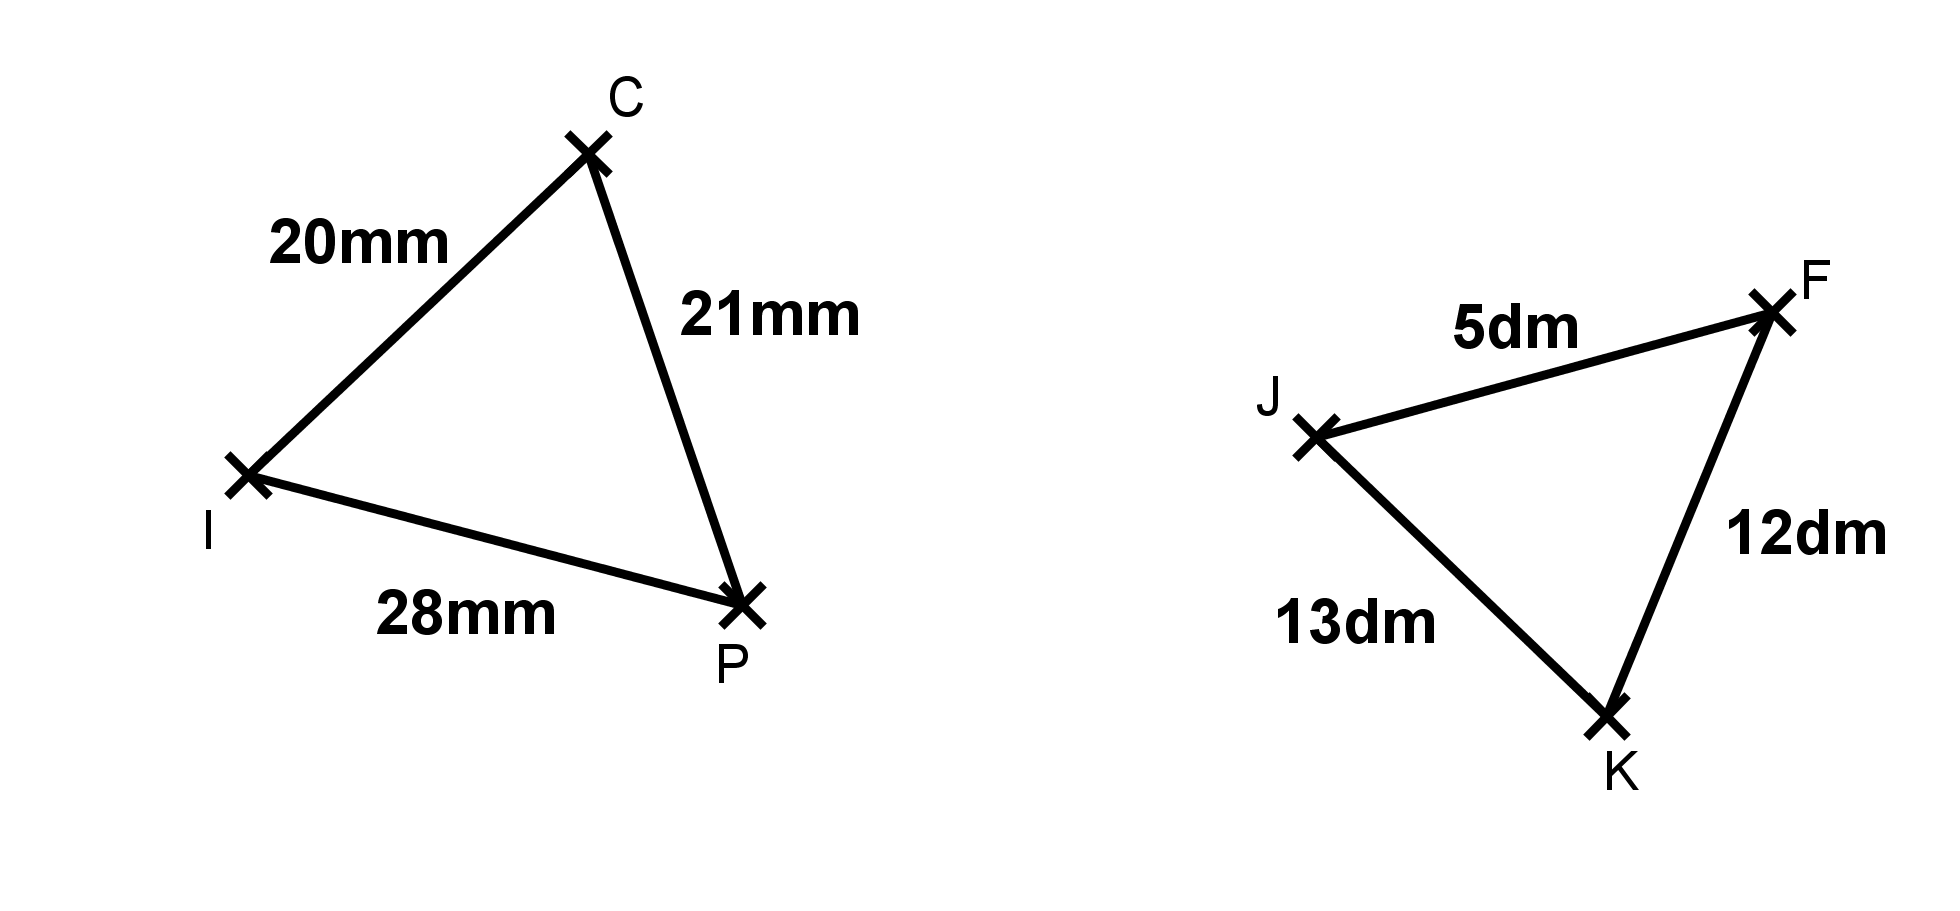
\includegraphics[width=10cm]{images/tri1.png} 
\end{center}






\subsection*{Exercice 3}


 
Un arbre s'est bris� en deux en tombant sur un mur de 2,5m de haut. Le pied de
l'arbre est situ� � 4m du pied du mur et la cime de l'arbre s'est retrouv� � 6m
du mur.

On cherche la hauteur totale de l'arbre.

\begin{tabular}{cc}
\begin{minipage}{10cm}
\begin{enumerate}
  \item Faire un sch�ma  en nommant les diff�rents points.
  \item Calculer la hauteur de l'arbre.
  \end{enumerate}
\end{minipage}
&
\begin{minipage}{8cm}
\qquad 
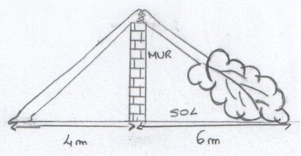
\includegraphics[width=65mm]{images/arbre.jpg}
\end{minipage}
\end{tabular}

\subsection*{Exercice 4}

Un parc de jeux a la forme d'un triangle DEF. Les dimensions r�elles du terrain
sont DE=12m, EF=9m et DF=15m.

\begin{enumerate}
  \item Construire le triangle DEF � l'�chelle $\dfrac{1}{200}$ (vous �crirez
  les calculs sur votre copie).
  \item Montrer que ce terrain poss�de un angle droit.
  \item Calculer l'aire r�elle de ce parc.
\end{enumerate}



\subsection*{Exercice 5}

Une lampe co�te 40 \euro. Pendant les soldes, le commer�ant baisse son prix de
25\%. Quelques jours plus tard, il d�cide de l'augmenter de 20\%.
\begin{enumerate}
  \item Quel est le prix final de la lampe?
  \item Calculer le pourcentage de r�duction.
\end{enumerate}
\end{document}
